
\section{Eigenschaften von Daten}


\begin{frame}
\frametitle{Strukturierte Daten}

\begin{itemize}
\item Menge von Datenobjekten
\item Objekte beschrieben durch ihre Eigenschaften (Attribute)
\item Attribut (Merkmal) vs. Attributwert (Ausprägung)
\begin{itemize}
\item ein Attribut $\longrightarrow$ verschiedene Attributwerte\\
z.B. Währung in \euro\ oder \$
\item verschiedene Attribute $\longrightarrow$ gleicher Attributwert\\
z.B. Kunden-Nr., Alter, Anzahl: \op{int}
\end{itemize}
\end{itemize}
\end{frame}

%---------------------------------------------------------------------

\begin{frame}
\frametitle{Attribute: Typen \& Eigenschaften}

\begin{itemize}
\item \hl{nominal}: Unterscheidung von Werten
\begin{itemize}
\item Bsp.: ID, PLZ, Geschlecht
\item Operationen: $=$, $\neq$
\end{itemize}
\item \hl{ordinal}: Festlegung einer Ordnung für Werte
\begin{itemize}
\item Bsp.: Zensur, Rang, Rating
\item Operationen: $=$, $\neq$, $<$, $>$
\end{itemize}
\item \hl{Intervall}: Differenz von Werten
\begin{itemize}
\item Bsp.: Datum, Zeit
\item Operationen: $=$, $\neq$, $<$, $>$, $+$, $-$
\end{itemize}
\item \hl{Ratio/Verhältnis}
\begin{itemize}
\item Bsp.: Menge, Anzahl, Länge
\item Operationen: $=$, $\neq$, $<$, $>$, $+$, $-$, $*$, $/$
\end{itemize}
\end{itemize}

\end{frame}

%---------------------------------------------------------------------

\begin{frame}
\frametitle{Diskrete vs. stetige Attribute}

\begin{itemize}
\item \hl{diskrete Attribute}
\begin{itemize}
\item endliche bzw. abzählbar unendliche Wertemenge
\item Datentyp: meist \op{integer}
\item Bsp.: Anzahl, Menge, PLZ, \dots
\end{itemize}
\item \hl{stetige bzw. kontinuierliche Attribute}
\begin{itemize}
\item reellwertiger Wertebereich
\item werden jedoch meist mit endlicher Anzahl von Stellen repräsentiert
\item Datentyp: \op{float}, \op{double}, \op{decimal}
\item Bsp.: Preis, Masse, Temperatur
\end{itemize}
\end{itemize}

\end{frame}

%---------------------------------------------------------------------


\begin{frame}
\frametitle{Satzorientierte Daten}

\begin{itemize}
\item Menge von Sätzen (Records) mit fester Attributmenge
\end{itemize}

{\small
\begin{tabular}{|c|c|c|c|c|}
\hline
\rowcolor{Gray} Kunden-ID & Schulden & Einkommen & Anstellungs- & Kredit- \\
\rowcolor{Gray}           &           &            & verhältnis   & würdigkeit \\
\hline\hline
1 & Hoch & Hoch & Selbständig & Schlecht \\
2 & Hoch & Hoch & Angestellt & Schlecht \\
3 & Hoch & Niedrig & Angestellt & Schlecht \\
4 & Niedrig & Niedrig & Angestellt & Gut \\
5 & Niedrig & Niedrig & Selbständig & Schlecht \\
6 & Niedrig & Hoch & Selbständig & Gut \\
7 & Niedrig & Hoch & Angestellt & Gut \\
\hline
\end{tabular}}

\end{frame}

%---------------------------------------------------------------------

\begin{frame}
\frametitle{Dokumentdaten}

\begin{itemize}
\item Dokumentrepräsentation als Vektor
\item Term (Schlüsselwort) repräsentiert Element im Vektor
\begin{itemize}
\item 0/1 für (Nicht-)Vorkommen
\item Häufigkeit des Vorkommens
\end{itemize}
\end{itemize}

\begin{center}
\begin{tabular}{|l|c|c|c|c|c|}
\hline
\rowcolor{Gray} & DBMS & KDD & Mining & Data & Web \\
\hline
\hline
Dokument \#1 & 3 & 2 & 0 & 1 & 0 \\
Dokument \#2 & 0 & 2 & 1 & 1 & 4 \\
Dokument \#3 & 0 & 0 & 2 & 4 & 3 \\
\hline
\end{tabular}
\end{center}

{\scriptsize
\begin{alltt}
\{"filter\_level":"medium","retweeted":false,\\
"{}in\_reply\_to\_screen\_name":"BeSassyChivette", \\
"possibly\_sensitive":false,"truncated":false,"lang":"{}en", \\
"id":553686454720032768,"timestamp\_ms":"1420844112459",\\
"created\_at":"Fri Jan 09 22:55:12 +0000 2015", \\
"text":"@BeSassyChivette gorgeous as usual", ... \}
\end{alltt}
}

\end{frame}

%---------------------------------------------------------------------

\begin{frame}
\frametitle{Transaktionsdaten}

\begin{itemize}
\item spezielle Form satzorientierter Daten
\item Datensatz entspricht Transaktion aus Transaktions-ID und Menge von Elementen (Items)
\end{itemize}

\begin{center}
\begin{tabular}{|c|l|}
\hline
\rowcolor{Gray} Transaktions-ID & Items \\
\hline
\hline
1 & Milch, Butter \\
2 & Milch, Honig, Butter \\
3 & Milch, Brot, Butter \\
4 & Milch, Brot, Honig \\
\hline
\end{tabular}
\end{center}


\end{frame}

%---------------------------------------------------------------------

\begin{frame}
\frametitle{Graphdaten}

\begin{itemize}
\item Graphstruktur, z.B. Web-Dokumente mit HTML-Links, soziale Netze, \dots
\end{itemize}

%\vspace*{-.5cm}
\begin{center}
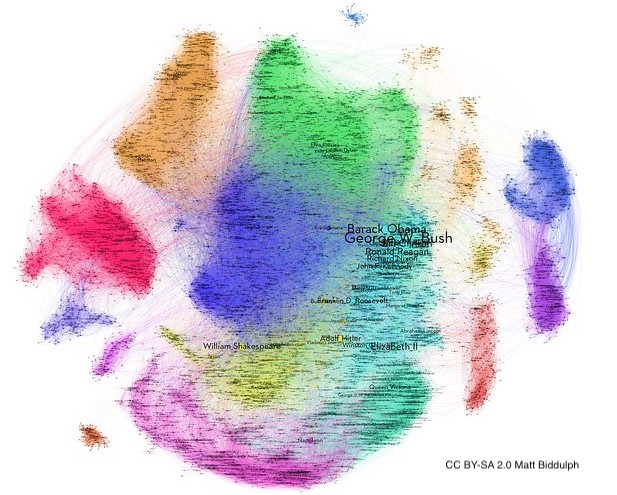
\includegraphics[scale=.35]{fig2/social-graph.jpg}
%{\tiny CC BY-SA 2.0 Matt Biddulph}
\end{center}
\end{frame}

%---------------------------------------------------------------------

\begin{frame}[fragile]
\frametitle{Ordnungsbasierte Daten}

\begin{itemize}
\item geordnete Folge von Elementen, z.B. Alarmmeldungen, Weblogs, Gensequenzen, spatio-temporale Daten
\end{itemize}

{\scriptsize
\begin{verbatim}
194.145.89.65 - - [19/Oct/2015:14:57:21 +0200] "GET ... HTTP/1.0"
194.145.89.65 - - [19/Oct/2015:14:57:21 +0200] "GET ... HTTP/1.0"
195.36.75.26 - - [19/Oct/2015:14:58:54 +0200] "GET ... HTTP/1.0"
195.37.152.250 - - [19/Oct/2015:15:02:55 +0200] "GET ... HTTP/1.1"
195.37.152.250 - - [19/Oct/2015:15:02:55 +0200] "GET ... HTTP/1.1"
193.51.91.2 - - [19/Oct/2015:15:06:20 +0200] "GET ... HTTP/1.0"
65.54.188.64 - - [19/Oct/2015:15:07:13 +0200] "GET ... HTTP/1.0"
84.168.66.17 - - [19/Oct/2015:15:12:02 +0200] "GET ... HTTP/1.1"
84.168.66.17 - - [19/Oct/2015:15:12:08 +0200] "GET ... HTTP/1.1"
68.142.251.148 - - [19/Oct/2015:15:22:14 +0200] "GET ... HTTP/1.0"
68.142.250.20 - - [19/Oct/2015:15:22:14 +0200] "GET ... HTTP/1.0"
\end{verbatim}
}

{%\scriptsize
\begin{verbatim}
ACAAGATGCCATTGTCCCCCGGCCTCCTGCTGCTGCTGCTCTCCGGGG
\end{verbatim}
}

\end{frame}

%---------------------------------------------------------------------

\section{Datenformate}

\begin{frame}
\frametitle{Datenformate}

\begin{itemize}
\item Kodierung von Daten mit mehreren Attributen
\item Zweck: Persistente Speicherung, Senden über das Netzwerk
\item Unterscheidung in textbasierte (menschenlesbare) und binäre Formate
\end{itemize}

\end{frame}

%---------------------------------------------------------------------

\begin{frame}[fragile]
\frametitle{Datenformate: CSV}

\begin{itemize}
\item \alert{C}omma-\alert{S}eparated \alert{V}alues
\item Daten lassen sich als Tabelle darstellen
\end{itemize}

\begin{lstlisting}
title,release_year
Duck the Halls: A Mickey Mouse Christmas Special,2016
Ernest Saves Christmas,1988
"Dr. Oakley, Yukon Vet",2013
\end{lstlisting}

\begin{itemize}
\item Trennung der Daten durch festgelegtes Zeichen (\code{\textbackslash{}n})
\item Trennung der Attribute durch anderes Zeichen (\code{,} \code{;} \code{\textbackslash{}t})
\item erste Zeile häufig für Namen der Attribute verwendet
\end{itemize}

\end{frame}

%---------------------------------------------------------------------

\begin{frame}[fragile]
\frametitle{Datenformate: JSON}

\begin{itemize}
\item \alert{J}ava\alert{S}cript \alert{O}bject \alert{N}otation
\item aus JavaScript Syntax entstanden
\item Parser für viele Sprachen verfügbar
\item Darstellung durch verschachtelte Objekte und Listen
\end{itemize}

\begin{lstlisting}[basicstyle=\tiny\ttfamily]
[
    {
        "title": "Duck the Halls: A Mickey Mouse Christmas Special",
        "cast": [
            "Chris Diamantopoulos",
            "Tony Anselmo",
            "Tress MacNeille",
            "Bill Farmer",
            "Russi Taylor",
            "Corey Burton"
        ]
    },
    {
        ...
    }
]
\end{lstlisting}

\end{frame}

%---------------------------------------------------------------------

\begin{frame}[fragile]
\frametitle{Datenformate: JSON}

\begin{itemize}
\item Das Dokument ist ein Objekt oder eine Liste.
\item Objekte werden von \code{\{\}} umschlossen und enthalten Schlüssel-Wert-Paare.
\item Listen werden von \code{[]} umschlossen und enthalten Werte.
\item Werte sind entweder primitive Datentypen oder selbst Objekte und Listen.
\end{itemize}

\begin{lstlisting}[basicstyle=\tiny\ttfamily]
[{
    "title": "Duck the Halls: A Mickey Mouse Christmas Special",
    "cast": [
        "Chris Diamantopoulos",
        "Tony Anselmo"
    ]
}, {
    ...
}]
\end{lstlisting}

\end{frame}

%---------------------------------------------------------------------

\begin{frame}[fragile]
\frametitle{Datenformate: Pickle}

\begin{itemize}
\item binäres Format
\item nur in Python verfügbar!
\end{itemize}

Vorteile binärer Formate:
\begin{itemize}
\item geringerer Speicherplatzverbrauch
\item schnelleres Serialisieren und Deserialisieren
\end{itemize}

Nachteile binärer Formate:
\begin{itemize}
\item strikte Einhaltung des Formats notwendig
\item Sicherheitsbedenken bei Deserialisierung
\item Ergebnisse nicht im Texteditor / optisch prüfbar
\end{itemize}

\end{frame}

%---------------------------------------------------------------------

\section{Der Data-Science-Prozess}

\begin{frame}[c]
\frametitle{Data-Science-Prozess: Überblick}

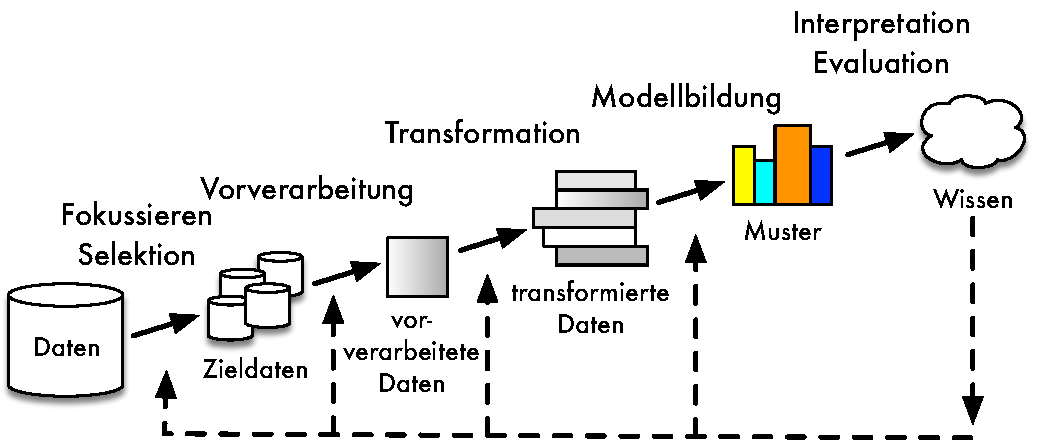
\includegraphics[scale=.6]{fig1/kdd-prozess.pdf}

\end{frame}

%---------------------------------------------------------------------

\begin{frame}
\frametitle{Prozess: Überblick /2}

\begin{itemize}
\item iterativer Prozess
\begin{itemize}
\item Selektion: Auswahl von Daten einer Datenbasis
\item Vorverarbeitung: Störungen wie Datenfehler oder
  Unvollständigkeit suchen und entfernen (entfällt beim Data Warehousing)
\item Transformation: Quantität verringern
\begin{itemize}
\item Attribute ohne oder mit geringem Vorkommen in der Datenbasis entfernen
\item in geeignete Analyseform umformen
\end{itemize}
\item Modellbildung: Aufgabenspezifikation bestimmt das Verfahren (statistische Verfahren, Data Mining, Machine Learning)
\item Interpretation und Verifikation
\end{itemize}
\end{itemize}


\end{frame}

%---------------------------------------------------------------------

\begin{frame}
\frametitle{Prozess: Fokussieren /Selektion}

\begin{itemize}
\item Auswahl der für die Analyseaufgabe notwendigen und relevanten Daten
\item ggf. Kampagne zur Datenerfassung notwendig
\item Beachtung der Datenqualität/-herkunft $\leadsto$ Vertrauenswürdigkeit, Grundprinzipien der Statistik
\item Vermeidung von Bias durch
\begin{itemize}
\item kognitive Verzerrungen (\url{https://de.wikipedia.org/wiki/Liste_kognitiver_Verzerrungen})
\item unvollständige Daten
\end{itemize}
\item Arbeit auf Dateien vs. ,,In-Database''-Analyse
\end{itemize}

\end{frame}

%---------------------------------------------------------------------

\begin{frame}
\frametitle{Prozess: Vorverarbeitung}

\begin{itemize}
\item Integration von Daten aus unterschiedlichen Quellen
\begin{itemize}
\item einfache Übersetzungen  von Attributnamen, z.B.\\
 \texttt{KNr} $\longrightarrow$ \texttt{KundenSchl}
\item Nutzen von Anwendungswissen um ähnliche Daten zusammenzufassen (z.B.
regionale Zuordnung von Postleitzahlen)
\end{itemize}
\item Konsistenzprüfung
\begin{itemize}
\item Test anwendungsspezifischer Konsistenzbedingungen
\item Bereinigung von Inkonsistenzen
\end{itemize}
\item Vervollständigung
\begin{itemize}
\item Ersetzen von unbekannten Attributwerten durch Defaults
\item Verteilung der Attributwerte soll i.A. erhalten bleiben!
\end{itemize}
\end{itemize}

\end{frame}

%---------------------------------------------------------------------

\begin{frame}
\frametitle{Prozess: Vorverarbeitung /2}

\begin{itemize}
\item Vorverarbeitung ist häufig einer der aufwendigsten Schritte -- bis zu 80\% des Gesamtaufwandes
\item wird häufig im Rahmen von Data-Warehouse-Systemen
durchgeführt
\end{itemize}

\begin{notebox}
\hl{Data Warehouse} :=
\begin{itemize}
\item \hl{dauerhafte}
\item \hl{integrierte} Sammlung von Daten
\item aus \hl{unterschiedlichen} Quellen
\item zum \hl{Zweck der Analyse} bzw. Entscheidungsunterstützung
\end{itemize}
\end{notebox}

\end{frame}

%---------------------------------------------------------------------

\begin{frame}
\frametitle{Data Warehousing: Prozess}

\begin{center}
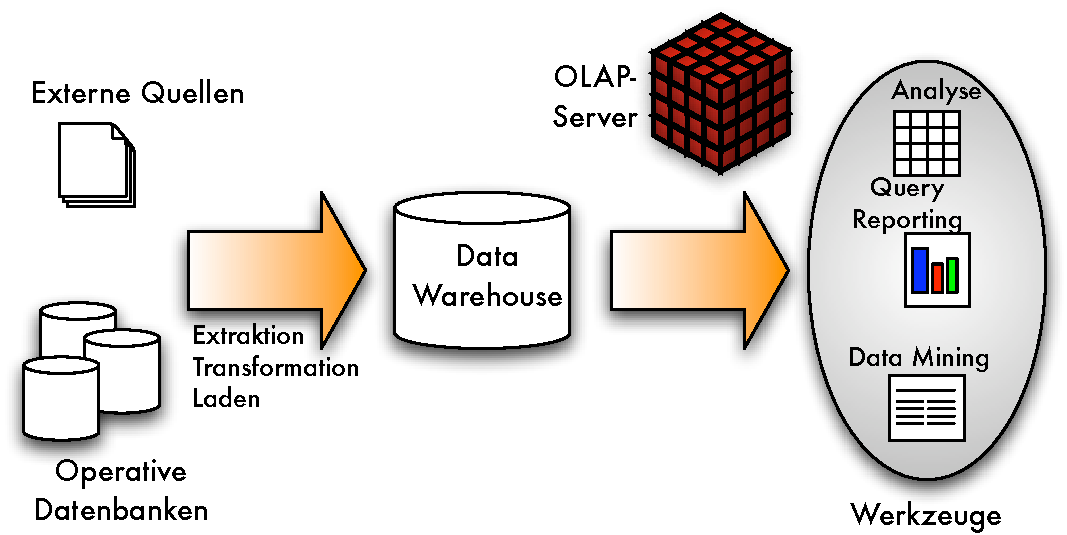
\includegraphics[scale=.6]{fig1/data-warehousing.pdf}
\end{center}

\end{frame}

%---------------------------------------------------------------------

\begin{frame}
\frametitle{Data Warehousing: Datenmodell}

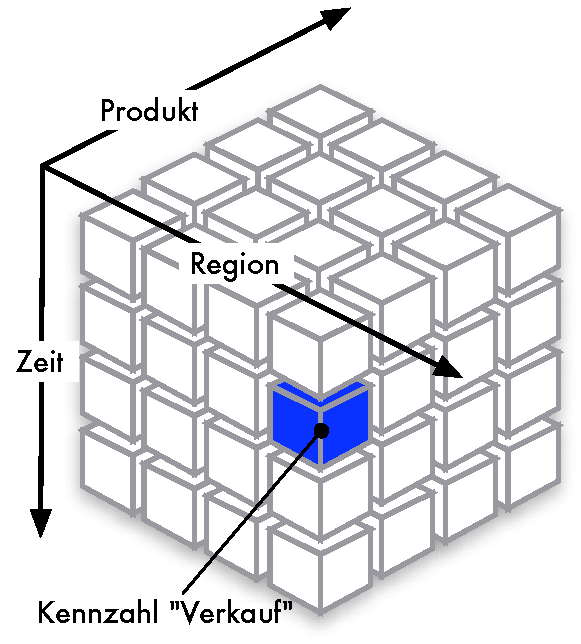
\includegraphics[scale=.4]{fig1/cube.pdf}\quad
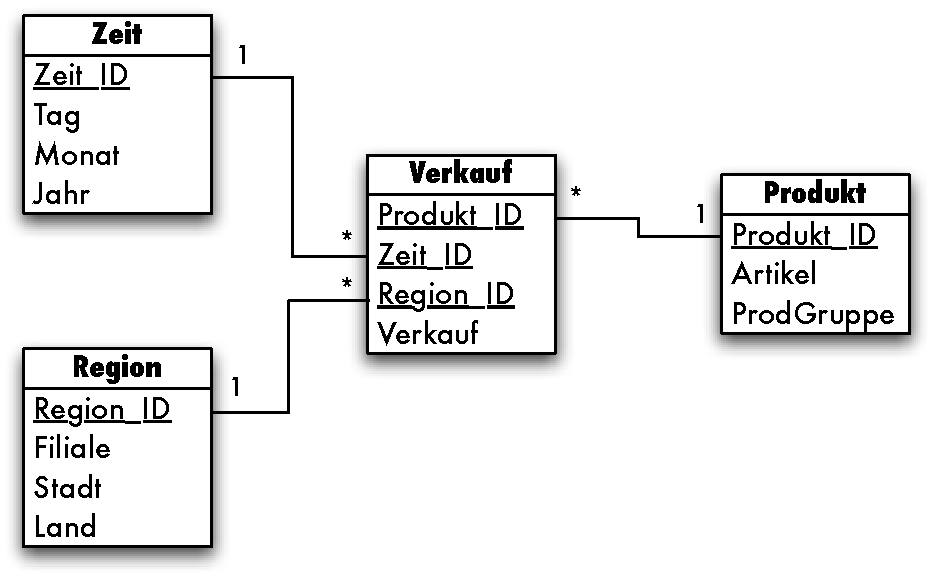
\includegraphics[scale=.4]{fig1/starschema.pdf}

\end{frame}

%---------------------------------------------------------------------

\begin{frame}
\frametitle{Prozess: Transformieren}

\begin{itemize}
\item Diskretisierung numerischer Attribute
\begin{itemize}
\item unabhängig von der Analyseaufgabe
z.B. Aufteilung des Wertebereichs in Intervalle gleicher Länge
\item abhängig von der Analyseaufgabe
z.B. Aufteilung in Intervalle so, dass der Informationsgewinn in Bezug auf die
Klassenzugehörigkeit maximiert wird
\end{itemize}

\item Erzeugen abgeleiteter Attribute / Feature-Extraktion
\begin{itemize}
\item durch Aggregation über Mengen von Datensätzen
z.B. von einzelnen Verkäufen zu "`Tagesumsatz, Wochenumsatz, Monatsumsatz"'
\item durch Verknüpfung mehrerer Attribute
z.B. Umsatzänderung = Umsatz 2018 - Umsatz 2017
\end{itemize}
\end{itemize}

\end{frame}

%---------------------------------------------------------------------

\begin{frame}
\frametitle{Prozess: Transformieren /2}

\begin{itemize}
\item Attribut-Selektion
\begin{itemize}
\item manuell:
\begin{itemize}
\item wenn Anwendungswissen über die Bedeutung der Attribute und über die
gegebene Datenanalyseaufgabe bekannt ist
\end{itemize}
\item automatisch:
\begin{itemize}
\item Bottom-Up (ausgehend von der leeren Menge jeweils ein Attribut
hinzufügen)
\item Top-Down (ausgehend von der Gesamtmenge der Attribute jeweils
  ein Attribut entfernen) z.B. so, dass die Diskriminierung der
  Klassen optimiert wird
\end{itemize}
\end{itemize}
\item Problem
\begin{itemize}
\item zu viele Attribute führen zu Ineffizienz und evtl. Ineffektivität
  des Data Mining
\item manche Transformationen können durch OLAP-Systeme realisiert
  werden
\end{itemize}
\end{itemize}

\end{frame}

%---------------------------------------------------------------------
\begin{frame}
  \frametitle{Prozess: Modellbildung}

  \begin{itemize}
    \item \hl{Ziel:} Ableitung eines Modells der Daten (=\hl{Abstraktion}) zur
    \begin{itemize}
      \item Beschreibung (für Aggregation/Generalisierung, Muster, Anomalieerkennung)
      \item Vorhersage
    \end{itemize}
        \item Methoden der klassischen Statistik: deskriptive, prädiktive und Inferenzstatistik
        \item \hl{Data Mining (statistische Verfahren)}
        \item Maschinelles Lernen, Deep Learning
      \end{itemize}

      \begin{center}
        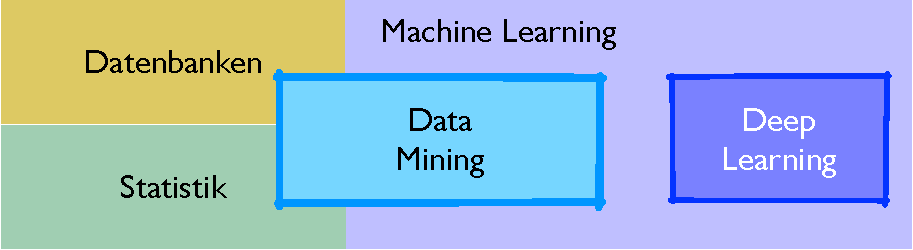
\includegraphics[scale=.6]{fig1/dm-vs-ml.pdf}
        \end{center}

\end{frame}
%---------------------------------------------------------------------

\begin{frame}
  \frametitle{Data Mining / Knowledge Discovery in Databases}

  Fayyad, Piatetsky-Shapiro \& Smyth
  \begin{notebox}
  Knowledge Discovery in Databases (KDD) ist der Prozess der (semi-)
  automatischen Extraktion von Wissen aus Datenbanken, das
  \hl{gültig}, \hl{bisher unbekannt} und \hl{potenziell nützlich} ist.
  \end{notebox}

  \begin{itemize}
  \item Anmerkungen
  \begin{itemize}
  \item (semi-)automatisch: im Unterschied zur manuellen Analyse, aber
    mit Nutzerinteraktion
  \item gültig: im statistischen Sinne
  \item bisher unbekannt: bisher nicht explizit vorhanden, kein
    "`Allgemeinwissen"'
  \item potenziell nützlich: für gegebene Anwendung
  \end{itemize}
  \end{itemize}

  \end{frame}



  %---------------------------------------------------------------------


\begin{frame}
  \frametitle{Data Mining}

  \begin{notebox}
  Data Mining ist die Anwendung effizienter Algorithmen, die die
    in der Datenbank enthaltenen Muster liefern
  \end{notebox}

  \begin{itemize}
  \item Prediktive Verfahren (Vorhersage):
  \begin{itemize}
  \item Nutzung von Merkmalen (Variablen) zur Vorhersage unbekannter
    oder zukünftiger Werte anderer Merkmale
  \item Beispiel: Klassifikation
  \end{itemize}
  \item Deskriptive Verfahren (Beschreibung):
  \begin{itemize}
  \item Extraktion von durch Menschen interpretierbare Muster, die die
    Daten beschreiben
  \item Beispiele: Assoziationsregeln, Clustering
  \end{itemize}
  \end{itemize}

  \end{frame}

  %---------------------------------------------------------------------


\begin{frame}
\frametitle{Prozess: Evaluation}

\begin{itemize}
\item Präsentation der gefundenen Muster: häufig durch entsprechende
  Visualisierungen
\item falls schlechte Bewertung (durch Benutzer): erneutes Data Mining mit
\begin{itemize}
\item anderen Parametern, anderem Verfahren, anderen Daten
\end{itemize}
\item falls gute Bewertung (durch Benutzer)
\begin{itemize}
\item Integration des gefundenen Wissens in die Wissensbasis
\item Nutzung des neuen Wissens für zukünftige KDD-Prozesse
\end{itemize}
\end{itemize}

\end{frame}

%---------------------------------------------------------------------

\begin{frame}
\frametitle{Prozess: Evaluation /2}

\begin{itemize}
\item Bewertung der gefundenen Muster
\begin{itemize}
\item Vorhersagekraft der Muster
\begin{itemize}
\item Verwendete Daten sind Stichprobe aus der Grundgesamtheit aller Daten.
\item Wie gut lassen sich die in diesen "`Trainingsdaten"' gefundenen
  Muster auf zukünftige Daten verallgemeinern?
\item Vorhersagekraft wächst mit Größe und Repräsentativität der Stichprobe.
\end{itemize}
\item Interessantheit der Muster
\begin{itemize}
\item Muster schon bekannt?
\item Muster überraschend?
\item Muster für viele Fälle anwendbar?
\end{itemize}
\end{itemize}
\end{itemize}

\end{frame}

%---------------------------------------------------------------------

\begin{frame}
  \frametitle{Data-Science-Stack}

  \begin{center}
    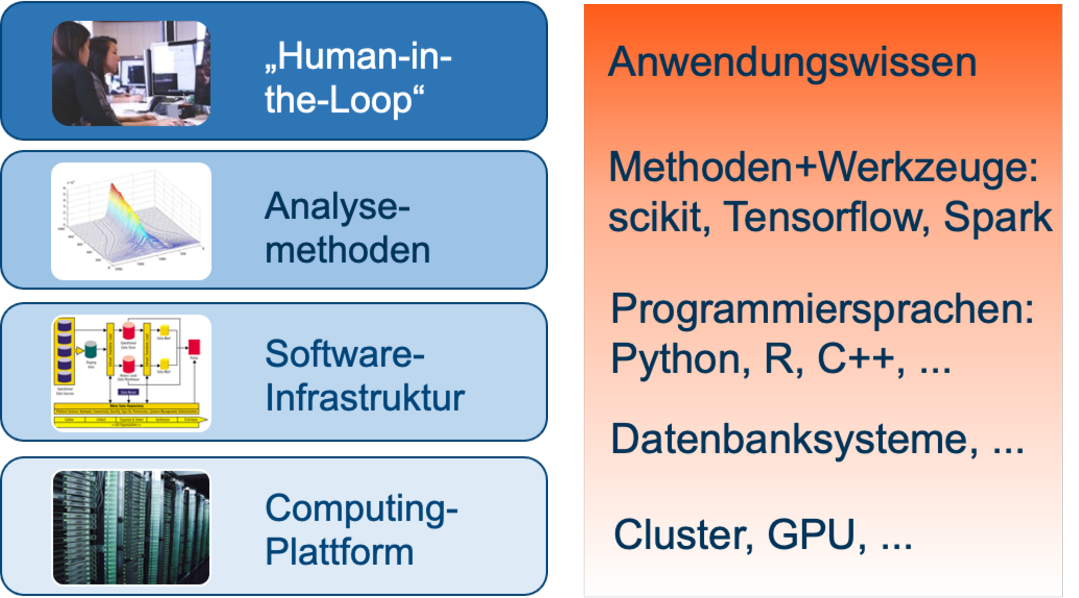
\includegraphics[scale=.6]{fig1/ds-stack.pdf}
    \end{center}

\end{frame}

%%%%%%%%%%%%%%%%%%%%%%%%%%%%%%%%%%%%%%%%%%%%%%%%%%%%%%%%%%%%%%%%%%%%%%

\section{Data-Science-Aufgaben}

\begin{frame}
\frametitle{Regression}

\begin{itemize}
\item Modellierung funktionaler Zusammenhänge zwischen unterschiedlichen Attributen
\item Schätzung unbekannter Werte mit entstehendem Modell
\item einfaches Modell der linearen Regression:  $y = mx + n$ (z.B. über Methode der kleinsten Quadrate)
\item für nichtlineare Zusammenhänge: z.B. durch Transformation der Daten über eine Basisfunktion, so dass Problem wieder linear ist
\end{itemize}

\vspace*{-.5cm}
\begin{center}
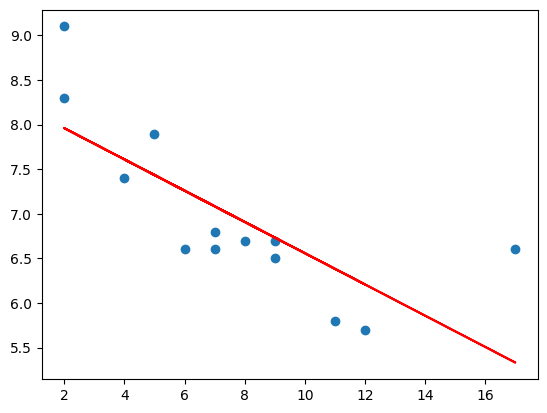
\includegraphics[scale=0.33]{fig1/linear_regression.png}
\end{center}

\end{frame}

%---------------------------------------------------------------------

\begin{frame}
\frametitle{Klassifikation: Beispiel}


\begin{itemize}
\item  Zuordnung von Objekten zu verschiedenen vorgegebenen Klassen,
  d.h. Vorhersage von Merkmalen (Klassenzuordnung) anhand anderer
  Merkmale
    \item Ableitung des \hl{Klassifikationsmodells} aus einer Trainingsmenge
% \item Beispiel: Kundenklassifikation bzgl. Schadensrisiko
%   (Kreditausfall)
\end{itemize}

\begin{center}
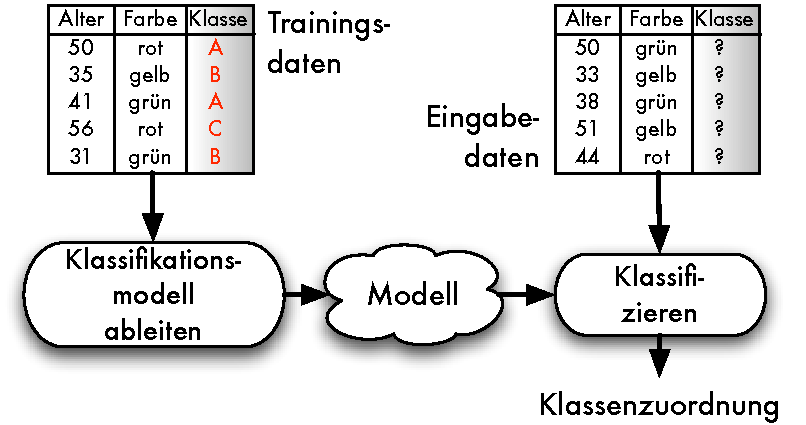
\includegraphics[scale=.6]{fig1/klassifikation-prinzip.pdf}
\end{center}

\end{frame}

%---------------------------------------------------------------------

\begin{frame}
\frametitle{Klassifikation: Beispiel /2}

{\tiny\begin{tabular}{|c|c|c|c|c|}
  \rowcolor{Gray}\hline
Kunden-ID & Schulden & Einkommen & Anstellungs- & Kredit- \\
\rowcolor{Gray}           &           &            & verhältnis   & würdigkeit \\
\hline\hline
1 & Hoch & Hoch & Selbständig & Schlecht \\
2 & Hoch & Hoch & Angestellt & Schlecht \\
3 & Hoch & Niedrig & Angestellt & Schlecht \\
4 & Niedrig & Niedrig & Angestellt & Gut \\
5 & Niedrig & Niedrig & Selbständig & Schlecht \\
6 & Niedrig & Hoch & Angestellt & Gut \\
7 & Niedrig & Hoch & Angestellt & Gut \\
\hline
\end{tabular}}

\raggedleft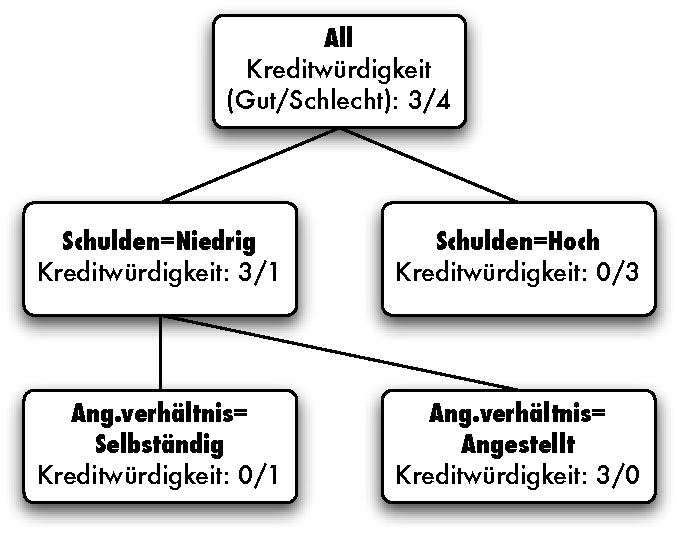
\includegraphics[scale=.5]{fig1/klassifikation.pdf}

\end{frame}

%---------------------------------------------------------------------

%\begin{frame}
%\frametitle{Assoziationsregeln: Beispiel}
%
%\begin{itemize}
%  \item Aufdeckung statistischer Zusammenhänge zwischen Variablen
%  \item Modell: Assoziationsregeln oder "`Frequent Itemsets"'
%\item Beispiel: Warenkorbanalyse
%\end{itemize}
%
%\begin{center}
%\begin{tabular}{|c|l|}
%\rowcolor{Gray}\hline
%Transaktions-ID & Produkte \\
%\hline
%\hline
%1 & Milch, Butter \\
%2 & Milch, Honig, Butter \\
%3 & Milch, Brot, Butter \\
%4 & Milch, Brot, Honig \\
%\hline
%\end{tabular}
%\end{center}
%\end{frame}

%---------------------------------------------------------------------

%\begin{frame}
%\frametitle{Assoziationsregeln: Beispiel /2}
%
%\begin{itemize}
%\item Frequent Itemsets
%
%{\small
%\begin{center}
%\begin{tabular}{|l|c|}
%  \rowcolor{Gray}\hline
%Produkte & Support \\
%\hline
%\hline
%\{ Milch \} & 4 \\
%\hline
%\{ Butter \}, & 3 \\
%\{ Milch, Butter \} & \\
%\hline
%\{ Honig \}, \{ Brot \}  & 2 \\
%\{ Honig, Milch \},
%\{ Brot, Milch \}  & \\
%\hline
%\end{tabular}\end{center}}
%
%\item Ableitung von Regeln:\\
%\fbox{\hl{Wenn ein Kunde Milch kauft, dann kauft er auch Butter.}}
%\begin{itemize}
%\item Unterstützung (Support): hier 3
%\item Konfidenz: hier 75\%
%\end{itemize}
%\end{itemize}
%
%\end{frame}

%---------------------------------------------------------------------

\begin{frame}[c]
\frametitle{Clustering: Beispiel}

\begin{minipage}[c]{5.5cm}
\begin{itemize}
\item Einordnung ähnlicher Objekte in neu gebildete Gruppen, so dass
\begin{enumerate}
\item Ähnlichkeit \hl{innerhalb} einer Gruppe möglichst \hl{groß},
\item Ähnlichkeit \hl{zwischen} Gruppen möglichst \hl{gering}
\end{enumerate}
\end{itemize}
\end{minipage}\quad
\begin{minipage}[c]{4cm}
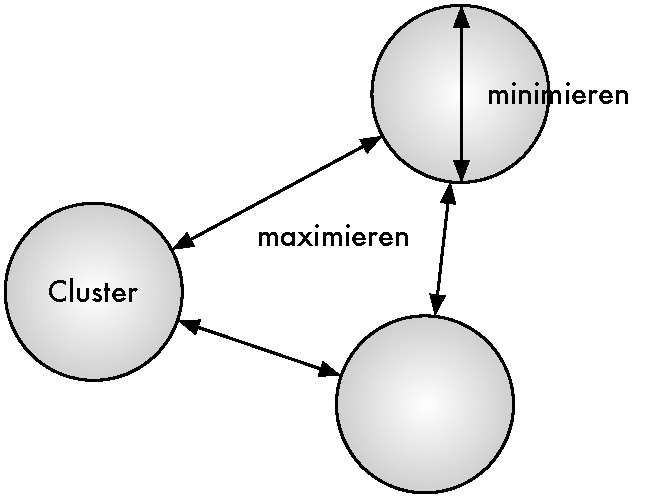
\includegraphics[scale=.5]{fig1/cluster.pdf}
\end{minipage}

\end{frame}

%---------------------------------------------------------------------

\begin{frame}[c]
\frametitle{Clustering: Beispiel /2}

\begin{minipage}[c]{3.5cm}
{\small\begin{tabular}{|c|r|}
  \rowcolor{Gray}\hline
Alter & Einkommen \\
\hline
\hline
\color{blue}{25} & \color{blue}{50.000} \\
\color{blue}{27} & \color{blue}{55.000} \\
\color{blue}{26} & \color{blue}{58.000} \\
\color{red}{40} & \color{red}{85.500} \\
\color{red}{42} & \color{red}{90.000} \\
\color{green}{57} & \color{green}{38.000} \\
\color{green}{59} & \color{green}{40.000} \\
\hline
\end{tabular}}
\end{minipage}\quad
\begin{minipage}[c]{6cm}
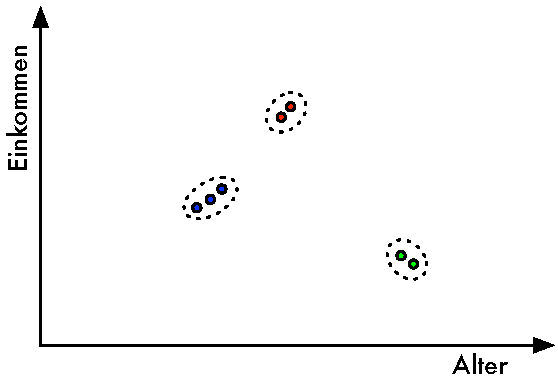
\includegraphics[scale=.7]{fig1/clustering.pdf}
\end{minipage}

\end{frame}

%---------------------------------------------------------------------

% \begin{frame}
% \frametitle{Sequenzanalyse}

% \begin{itemize}
% \item Suche nach häufig auftretenden Episoden oder Ereignisfolgen in
%   Datenbeständen mit (zeitlicher) Ordnung
% \begin{itemize}
% \item Menge von Ereignistypen $E$, Sequenz von Paaren $(e, t$) mit $e
%   \in E$ und $t$ ist Zeitstempel
% \item Episode $\alpha$: partielle Ordnung von Ereignistypen
% \item Häufigkeit einer Episode $\alpha$: Anzahl der Partition der
%   Sequenz einer vorgegebenen Länge mit den durch $\alpha$ gegebenen
%   Ereignistypen und deren Ordnung
% \end{itemize}

% \item Anwendungen
% \begin{itemize}
% \item Analyse von Alarmmeldungen (Events) in
%   Telekommunikationssystemen
% \item Web Usage Mining / Clickstream-Analyse
% \item (zeitliches) Kaufverhalten, z.B.
%  "`Herr der Ringe (DVD)"'
%   $\longrightarrow$ "`Herr der Ringe (Buch)"' $\longrightarrow$
%   "`Silmarillion"'
% \end{itemize}
% \end{itemize}

% \end{frame}

%---------------------------------------------------------------------

\begin{frame}
\frametitle{Graph Mining: Analyse sozialer Netzwerke}

\begin{itemize}
\item Freundschaftsbeziehungen in sozialen Netzen wie Facebook,
  Follower in Twitter, \dots
\end{itemize}

\begin{minipage}[c]{4.5cm}
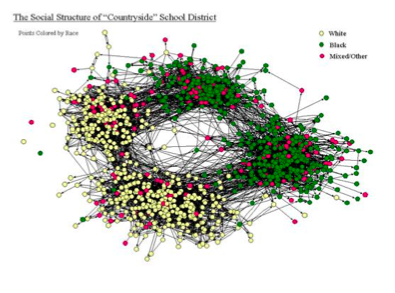
\includegraphics[width=4.5cm]{fig1/graph.png}
\end{minipage}\quad
\begin{minipage}[c]{5.5cm}
{\small
\begin{itemize}
\item Auffinden von Communities: Gruppen mit starken innerem
  Zusammenhang
\item Identifzieren von Autoritäten: wichtige Knoten/Peers (Personen)
  im Netzwerk
\item Link-Vorhersage und virales Marketing: Modellierung und
  Vorhersage von Diffusionsprozessen
\end{itemize}}
\end{minipage}

\end{frame}

%---------------------------------------------------------------------

\begin{frame}
\frametitle{Weitere Aufgabenstellungen}

\begin{itemize}
\item \hl{Text Mining:} Analyse von un- oder schwachstrukturierten Textdaten zur Aufdeckung von Semantik und Strukturen
\begin{itemize}
\item Dokumentenrepräsentation und Dokument-Clustering
\item Informationsextraktion: Entity Recognition, Sentiment-Analyse, \dots
\item Natural Language Processing
\end{itemize}
\item \hl{Spatio-Temporal Mining:} Analyse von Daten mit räumlichem
  und/oder zeitlichem Bezug
\begin{itemize}
\item Muster: räumliche Ausreißer (z.B. Stauzonen in Verkehrsnetzen),
  Vorhersage von Lokation/Bewegung (zur Optimierung von
  Transportsystemen), räumliche Cluster, Ko-Lokationen
\end{itemize}
\end{itemize}
\end{frame}


%---------------------------------------------------------------------

\begin{frame}
\frametitle{Zusammenfassung}

\begin{itemize}
\item \hl{Daten} als Analyseobjekte
\item Grundlagen des \hl{Data-Science-Prozesses}
\item typische \hl{Analyseaufgaben}
\begin{itemize}
\item Regression
\item Klassifikation
\item Clustering
\item \dots
\end{itemize}
\end{itemize}

\end{frame}

%---------------------------------------------------------------------

%%% Local Variables:
%%% mode: latex
%%% TeX-master: "main"
%%% End:
